\documentclass[12pt]{book}

\usepackage{amsmath}
\usepackage{amssymb}
\usepackage{amsthm}
\usepackage{graphicx}
\usepackage{listings}

\theoremstyle{definition}
\newtheorem{definition}{Definition}

\theoremstyle{plain}
\newtheorem{corollary}{Corollary}
\newtheorem{lemma}{Lemma}
\newtheorem{theorem}{Theorem}

\lstset{
    basicstyle=\ttfamily
}

\title{An Introduction to the Aptos Blockchain}
\author{Brent A. Ritterbeck}
\date{\today}

\begin{document}
\maketitle

\chapter{The Aptos CLI}

\begin{lstlisting}[caption={Creating a Default Profile}]
aptos init
\end{lstlisting}

\begin{figure}[htp]
\centering
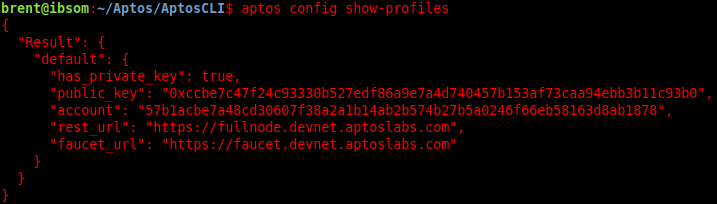
\includegraphics[scale=0.50]{./images/default_profile.png}
\caption{Default Profile}
\end{figure}

\begin{lstlisting}[caption={Creating a Named Profile}]
aptos init --profile Alpha
\end{lstlisting}

\begin{lstlisting}[caption={Show Initial Project Options}]
aptos move init --help
\end{lstlisting}

\begin{lstlisting}[caption={Create Project Shell}]
aptos move init --package-dir Transfer --name Transfer
\end{lstlisting}

\begin{lstlisting}[caption={Create Sender Profile}]
aptos init --profile Sender
\end{lstlisting}

\begin{lstlisting}[caption={Create Receiver Profile}]
aptos init --profile Receiver
\end{lstlisting}

\end{document}
